\graphicspath{{Kapitel/Kapitel2_Grundlagen/Images/}}

Dieses Kapitel befasst sich mit einigen grundlegenden Themen, die mit dem Inhalt dieser Arbeit zu tun haben. Dies soll dem besseren Verständnis für die folgenden Kapitel dienen. Der Abschnitt \ref{sec:Lidar} beispielsweise, erläutert die Art und Weise, wie Punktwolken mittels eines LiDAR-Sensors erfasst werden. Damit soll verdeutlicht werden, was Punktwolken für eine Bedeutung haben und wie sie entstehen. Das Kapitel \ref{sec:AnnotationIntro} befasst sich mit der Annotation von Daten im Bereich des maschinellen Lernens. Darin wird der Prozess des maschinellen Lernens erläutert, um zu verdeutlichen, was Annotation von Daten in diesem Prozess für eine Bedeutung hat. Anschließend wird konkret auf die Annotation von Punktwolken eingegangen. Da im Zuge dieser Arbeit eine Virtual Reality Applikation entwickelt wurde, wird im Abschnitt \ref{sec:VirtualReality} auch das Thema Virtual Reality im Allgemeinen behandelt.

\section{Erfassung von Punktwolken mit LiDAR}
\label{sec:Lidar}

Punktwolken, wie sie in dieser Arbeit behandelt werden, bestehen aus vielen einzelnen Abstandsmessungen, wobei jeder Punkt einer dieser Messungen entspricht. LiDAR (\textit{Light Detection and Ranging}) ist eine Methode zur Abstandsmessung mit Hilfe von Licht, welche in der Automobilbranche häufig verwendet wird. In den letzten Jahrzehnten wurde der LiDAR-Sensor aber auch in vielen anderen Bereichen zur herkömmlichen Methode, wenn es um die Messung von Abstandsinformationen geht. Im Bereich Archeologie benutzten Johnson und Oiumet diese Technologie, um die Landschaft von New England in den USA zu analysieren \cite{bib:LidarArcheology}. Die Analyse von Landschaften ist durch LiDAR aber nicht nur auf dem Planeten Erde möglich. In \cite{bib:LidarSpace} wurde LiDAR benutzt um Oberflächenmessungen auf dem Mars durchzuführen. In der Robotik wird es häufig verwendet um Hindernisse für mobile Roboter zu identifizieren, wie in \cite{bib:LidarRobotic}.\\

Für die Messung der Distanz wird in der Regel ein Laser benutzt. Der LiDAR-Sensor sendet mit Hilfe eines solchen Lasers einen Lichtimpuls aus und misst die Zeit $t$ bis das Signal wiederkehrt. Anhand dieser Zeit ist es möglich die Distanz $d$ zu bestimmen, die vom Licht zurückgelegt wurde. Dazu nimmt man die Formel \ref{eq:LidarDistance}, in der $c$ für die Geschwindigkeit des Lichts steht.

\begin{equation}
\label{eq:LidarDistance}
\ d = \frac{c\cdot\Delta t}{2}
\end{equation} 

Mit dem Impuls eines einzelnen Lasers bekommt man eine einzelne Abstandsmessung für den Zeitpunkt des Impulses. Führt man aber viele dieser Messungen innerhalb einer 360° Drehung durch bekommt man Abstandsinformationen des gesamten Umfeldes. Eine Möglichkeit eine 360° Umfeldmessung zu ermöglichen ist es, den Sensor um seine eigene Achse zu drehen, wie es in Abbildung \ref{fig:Lidar} gezeigt wird. In der oberen Reihe dieser Abbildung ist der LiDAR-Sensor zu sehen, dessen Lichtimpuls durch einen Spiegel (graues Objekt) gezielt auf die Umgebung gerichtet wird. Dieser Spiegel dreht sich um die eigene Achse um die Lichtimpulse nach und nach auf das Umfeld zu verteilen. In der mittleren Reihe ist die Vogelperspektive auf den Sensor und seine Umgebung abgebildet. Der Sensor ist, wie in der oberen Abbildung, in blau dargestellt und die Objekte des Umfeldes in grün. Die unteren Abbildungen zeigen, ebenfalls in der Vogelperspektive, die Abstandsinformationen, die der Sensor liefert. Diese werden in Form von blauen Punkten dargestellt und bilden eine zweidimensionale Punktwolke, in der man den Rahmen des Umfelds und das kreisförmige Objekt erkennen kann.\\

\begin{figure}%
    \centering
    \subfloat[]{{\includegraphics[width=4cm]{Lidar1}\label{fig:Lidar1}}}%
    \qquad
    \subfloat[]{{\includegraphics[width=4cm]{Lidar2Phi}\label{fig:Lidar2}}}%
    \qquad
    \subfloat[]{{\includegraphics[width=4cm]{Lidar3}\label{fig:Lidar3}}}%
    \caption{Ablauf einer LiDAR-Messung von einem Sensor, der die Messimpulse im Uhrzeigersinn abgibt. Die Bilder stammen von \cite{bib:LidarPictures} und \ref {fig:Lidar2} wurde um den Winkel $\varphi$ erweitert.}\label{fig:Lidar}%
\end{figure}

Diese Methode liefert also eine gute horizontale Rundumsicht, welche aber innerhalb der vertikalen Sichtweite keinerlei Informationen bietet. Dies genügt in der Regel für simple Abstandserkennungen und Detektion von Hindernissen auf Höhe des Sensors. Möchte man jedoch Aussagen über das Detektierte treffen oder braucht Informationen über andere vertikalen Ebenen, beispielsweise den Boden, muss man diese Methode noch erweitern. Dafür werden mehrere Lichtimpulse mit verschiedenen vertikalen Winkeln ausgesendet. Diese treffen die Umgebung dann mit unterschiedlicher Höhe womit die daraus resultierende Punktwolke eine dritte Dimension erhält. In Abbildung \ref{fig:LidarVertical} ist die seitliche Sicht auf einen LiDAR-Sensor mit mehreren vertikalen Lasern zu sehen.\\

\begin{figure}%
	\centering
    \includegraphics[width=14cm]{LidarVerticalTheta}
    \caption{Seitliche Sicht auf eine LiDAR-Messung mit mehreren, verital angeordneten Lasern. Die Abbildung stammt aus \cite{bib:FastGroundSeg} und wurde durch die Einzeichnung des Winkels $\theta$ erweitert.}
    \label{fig:LidarVertical}
\end{figure}

Wie schon erwähnt werden die erhaltenen Messdaten in eine Struktur konvertiert, die sich Punktwolke nennt. Dafür werden die Abstandsinformationen innerhalb eines bestimmten Koordinatensystems dargestellt. In der Regel wird dabei das \textit{Sphärische Koordinatensystem} verwendet. Darin wird jeder Punkt durch einen Abstand $r$ von einem Referenzpunkt und zwei dazugehörigen Winkel repräsentiert. Einer dieser Winkel ist dabei horizontal (Winkel $\varphi$) zu interpretieren und der andere vertikal (Winkel $\theta$). 

Nimmt man den Punkt \glqq 1\grqq{} aus der Abbildung \ref{fig:LidarVertical} als Beispiel, entspräche $\theta$ dem vertikalen Winkel. Dieser gibt den Winkel zwischen der gelben, gestrichelten Linie und der roten Linie an, die den Sensor und \glqq 1\grqq{} verbindet. Diese rote Linie repräsentiert den Abstand des Punktes vom Referenzpunkt, welcher der Position des Sensors entspricht. Der horizontale Winkel ist der Rotationswinkel des Sensors um seine eigene Achse (vgl. $\varphi$ in Abbildung \ref {fig:Lidar2}). Dieser wird vom Sensor bei jedem abgegebenen Impuls gemessen. Zusammenfassend kann also durch den vertikalen Winkel $\theta$ des Lichtimpulses, den horizontalen Winkel $\varphi$ des Sensors und dem gemessenen Abstand $r$ zum Sensor, der Punkt \glqq 1\grqq{} genau im Raum definiert werden.\\

Viele Anwendungen, die mit Punktwolken zu tun haben arbeiten jedoch mit dem kartesischen Koordinatensystem, so auch C.LABEL-VR. In diesem Koordinatensystem wird jeder dreidimensionale Punkt durch drei Koordinaten angegeben, nämlich der $x$-, $y$- und $z$-Koordinate. Ausgehend von den drei Werten des sphärischen Koordinatensystem können die drei kartesischen Koordinaten durch die Formeln in \ref{eq:SphToKart} berechnet werden. Auch hier steht $r$ für den Abstand zwischen dem Referenzpunkt und dem Punkt den man definieren will. $\theta$ steht für den vertikalen Winkel und $\varphi$ für den horizontalen Winkel, also den Rotationswinkel des Sensors um die eigene Achse.

\begin{subequations}
\begin{align}
        &x = r\sin\theta\cos\varphi \\
		&y = r\sin\theta\sin\varphi \\
		&z = r\sin\theta
\end{align}
\label{eq:SphToKart}
\end{subequations}

Durch die eben erklärte Definition der Messdaten in einem Koordinatensystem können diese Daten nun mit geeigneten Programmen (C.LABEL) als Punktwolke dargestellt werden. Darin ist dann jede einzelne Messung die der Sensor getätigt hat sichtbar. Somit kann der Mensch die Daten visuell analysieren und beispielsweise Zusammenhänge wie Objekte entdecken. Damit auch Computersysteme solche Objekte in diesen Daten erkennen können müssen sie erst lernen wie diese aussehen. Dazu muss eine Vielzahl an Punktwolken mit Hilfe eines LiDAR-Sensors aufgenommen werden und anschließend eine, vom Anwendungsfall abhängige, Anzahl an Punkten in dieser Wolke mit entsprechenden Klassifikationen versehen werden (Prinzip der Annotation aus Kapitel \ref{sec:Annotation}). Mit den annotierten Daten können nun Algorithmen, wie beispielsweise künstliche neuronale Netze (vgl. Kapitel \ref{sec:KNN}), lernen welche Zusammenhänge es in solchen Daten gibt und diese dann in nicht annotierten Daten wiedererkennen. Das Ziel von C.LABEL-VR ist es solche Daten in der virtuellen Realität zu visualisieren und Funktionen zur Verfügung zu stellen diese in der virtuelle Umgebung zu annotieren.

\section{Datenannotation im Bereich des maschinellen Lernens}
\label{sec:AnnotationIntro}

Um den Grund und die Wichtigkeit der Datenannotation, im Bereich des maschinellen Lernens zu verstehen, ist es hilfreich den Prozess des maschinellen Lernens selbst zu verstehen. Beim maschinellen Lernen, geht es in der Regel darum, dass ein Computersystem eine bestimmte Aufgabe löst, in dem es zuvor erhaltenes Wissen und gemachte Erfahrungen anwendet, um diese Aufgabe zu lösen. Dazu soll das System aus relevanten Trainingsdaten Muster und Gesetzmäßigkeiten erkennen, um diese dann auf unbekannte Daten zu verallgemeinern. Das System lernt also aus lehrreichen Daten das lösen eines Problems und kann das gelernte dann auf unbekannte Daten anwenden. Um die Trainingsdaten für diesen Prozess so aussagekräftig wie möglich zu machen, müssen alle relevanten Inhalte der Daten richtig gekennzeichnet werden. Möchte man beispielsweise ein System auf die Erkennung von Gesichtern trainieren, wie es bei handelsüblichen Smartphone-Kameras der Fall ist, müssen in den Trainingsdaten, die in diesem Fall Bilder sind, alle Gesichter gekennzeichnet werden. Eine solche Kennzeichnung nennt sich \textit{Label}. Das erstellen solcher Labels nennt sich Annotation. Im Folgenden soll der Prozess des maschinellen Lernens und der Datenannotation genauer erläutert werden. Anschließend wird konkret auf die Annotation von 3D-Punktwolken eingegangen.

\subsection{Maschinelles Lernen}
\label{sec:MLearning}
Der Ausdruck Maschinelles Lernen (engl.: \textit{Machine Learning}) ist heutzutage ein Überbegriff für Methoden, die versuchen durch Optimierung eine Funktion zu erlernen. Bei solch einer Funktion kann es sich sowohl um eine simple binäre Entscheidung auf eine Fragestellung handeln als auch um komplexere Dinge wie das Übersetzen von Texten in eine andere Sprache, das Erkennen von Personen auf Bildern, oder eben das Klassifizieren von Objekten in einer Punktwolke. Letzteres ist speziell für diese Arbeit relevant. Die Komplexität der Funktion bestimmt auch die zu verwendende Methode zur Lösung des Problems. Im Zuge des \textit{Azure Machine Learning Studios} veröffentlichte Microsoft eine Grafik (vgl. Abbildung \ref{fig:MLCS}), mit der man den richtigen Lernalgorithmus für gewisse Vorhersage-Methoden bestimmen kann. Für die Objektklassifizierung im Automobilbereich ist es wichtig die Klasse eines Objekts mit hoher Genauigkeit aus einer großen Anzahl verschiedener Klassen zu bestimmen. Basierend auf der Grafik \ref{fig:MLCS} ist die beste Methode dafür die Verwendung eines künstlichen neuronalen Netzes (KNN). Die Benutzung solcher Netze ist üblich, wenn es um Klassifikation von vielen verschiedenen Dingen geht und soll im Folgenden näher erläutert werden.\\

TODO BILD Grafik von Bild- und Wolkenerkennung\\

\begin{figure}%
	\centering
    \includegraphics[width=19cm, angle=270]{MLCS}
    \caption{Diagramm um den besten Machine Learning Algorithmus für eine \gls{glos:PredAna}-Methoden zu finden \cite{bib:AzureCs}}
    \label{fig:MLCS}
\end{figure}
  
\subsubsection{Künstliche Neuronale Netze}
\label{sec:KNN}
David Kriesel hat in \cite{bib:UebereblickNN} den Zusammenhang zwischen physischen und künstlichen neuronalen Netzen dargestellt. Seine Arbeit soll im Folgenden als Quelle dienen. Das Prinzip der künstlichen neuronalen Netze ist, wie vieles in der Informatik, einer Struktur aus der realen Welt nachempfunden. Das komplexeste neuronale Netz ist wohl das menschliche Gehirn mit etwa 86 Milliarden Nervenzellen, welche auch Neuronen genannt werden. Daher kommt auch der Begriff des neuronalen Netzes. Diese Nervenzellen sind durch Synapsen mit bis zu mehreren Tausend anderen Zellen verbunden. Diese Verbindungen bilden zusammen das Netz. Die Kommunikation zwischen den Neuronen erfolgt in der Regel über elektrische Impulse und chemische Botenstoffe \ref{fig:Neurons}. Beides wird über Synapsen zu den nächsten, verbundenen Neuronen weitergeleitet und bewirkt dort einen Reiz. Durch Übertragung von chemischen Botenstoffen kann dieser Reiz zusätzlich gewichtet werden, das heißt es kann ein stärkerer oder schwächerer Reiz ausgesendet werden. Alle ankommenden Reize werden dann am Empfangsneuron akkumuliert und ergeben den Eingangsreiz des Neurons.\\ 

Dieses, vereinfacht dargestellte Prinzip, wird auch bei den \acrshort{acr:knn}s verwendet. Übersteigt dieser Reiz eine bestimmte Schwelle kommt es zum entscheidenden Ereignis: Das Neuron \textit{feuert}. Dadurch gibt das feuernde Neurone einen Impuls an alle anderen Neuronen weiter mit dem es verbunden ist. Bei dafür vorgesehenen Neuronen oder verbänden davon, kann dieser Impuls auch ein Ereignis auslösen. Diese Ereignisse können physischer Natur sein, also beispielsweise Bewegungen, oder auch psychischer Natur, zum Beispiel das Erkennen von Dingen. Werden diese Nervenzellen also mit einem ausreichenden Impuls angesprochen, wird das entsprechende Ereignis ausgelöst.\\

\begin{figure}%
	\centering
    \includegraphics[width=9cm]{Neurons}
    \caption{Abbildung des Übertragungsprinzips von Reizen zwischen Neuronen \cite{bib:Neurons}}
    \label{fig:Neurons}
\end{figure}

Die entscheidende Komponente dieses Prinzips ist die adaptive Gewichtung der weitergegebenen Reize. Adaptiv deswegen, da die Gewichtung der Reize sich während eines Menschenlebens verändern können. So erkennen Kinder oft Gefahrensituation nicht, da ihr Gehirn nicht ausreichend geschult ist, um diese zu erkennen. In diesem Kontext bedeutet das, dass an die \textit{Gefahren-Neuronen} kein ausreichend starker Reiz gesendet wird. Durch sammeln von Erfahrungen optimiert sich dieser Wert, was in späteren Jahren zu einer anderen Reaktion des Gehirns führen kann als früher. Das Adaptieren dieser Gewichte auf einen passenden Wert bezeichnen wir als Lernen. Um Computersystemen einen derartigen Lerneffekt zu ermöglichen wurde dieses Biologische Prinzip nun mathematisch imitiert. \\

\begin{figure}%
	\centering
    \includegraphics[width=13cm]{Perceptron}
    \caption{Einfaches Perzeptron nach dem Prinzip von Frank Rosenblatt}
    \label{fig:Perceptron}
\end{figure}

Künstliche Neuronale Netze basieren auf dem Prinzip des Perzeptrons, das von Frank Rosenblatt 1958 vorgestellt wurde \cite{bib:Perzeptron}. Dieses Perzeptron repräsentiert die Funktion eines einzelnen Neurons auf eine mathematische Weise (vgl. \ref{fig:Perceptron}). Die Eingangsdaten eines Perzeptrons bestehen aus einer \(n\)-großen Menge an Werten \(x_1 \dots x_n\), welche eine gleichgroße Menge an jeweiligen Gewichten \(W_1 \dots W_n\) haben. Wenn das zu analysierende Ziel beispielsweise ein Bild ist, wäre \(n\) die Menge aller Pixel des Bildes und bei Punktwolken eben die Anzahl der Punkte. Die Eingangswerte werden von einer mathematischen Funktion empfangen und zu einem skalaren Wert \(z\) zusammengefasst. Hierbei wird meist die Gewichtete Summe benutzt die folgendermaßen berechnet wird:

\begin{equation}
z = \sum \limits_{i=0}^{n} W_i \cdot x_i
\end{equation}\\

Im biologischen Vorbild repräsentiert diese Summe den eingehenden Reiz in eine Nervenzelle, die \(x\)-Werte sind dabei die Impulse der vorherigen Neuronen und die \(W\)-Werte repräsentieren die Gewichtung, also die Stärke der Eingangsreize. Der biologische Schwellwert wird im Perzeptron durch eine Mathematische Funktion \(\sigma(z)\) dargestellt. Wie in \cite{bib:NeuronaleNetze} beschrieben gibt es dafür zwei beliebte Funktionen. Die \textit{Fermifunktion} (\ref{eq:Fermi}) , auch Logische Funktion genannt, welche einen Ausgabe-Wertebereich von (0,1) hat und den \textit{Tangens Hyperbolicus} (\(tanh(z)\)) mit einem Wertebereich von (-1,1). Beide sind differenzierbar, was wichtig für das Lernen mit \textit{Backpropagation} ist. Was das bedeutet wird in Abschnitt \ref{sec:Training} näher erläutert. Wenn der Wert, den diese Funktion liefert, nicht noch durch eine weitere Ausgangsfunktion verändert wird, ist er der Ausgangswert des Perzeptrons.

\begin{equation}
\sigma(z) = \frac{1}{1 + e^{-z}}
\label{eq:Fermi}
\end{equation}

In \acrshort{acr:knn}s können mehrere dieser Perzeptrons eine sogenannte Schicht bilden. Je mehr Schichten ein neuronales Netz hat desto \textit{tiefer} ist es, daher auch der Begriff \textit{Deep Learning}, also tiefes Lernen. In der Regel bestehen \acrshort{acr:knn}s aus mindestens 3 Schichten, nämlich einer Eingangsschicht, einer oder mehrerer Zwischenschichten und einer Ausgangsschicht (veranschaulicht in Abbildung \ref{fig:Bilderkennung}). Die einzelnen Schichten werden im Folgenden kurz erläutert.  

\begin{itemize}
\item \textbf{Eingangsschicht}\\
Die Eingabeschicht ist der Startpunkt des Informationsflusses in einem künstlichen neuronalen Netzes. Eingangssignale werden von den Neuronen dieser Schicht aufgenommen und gewichtet an alle Neuronen der ersten Zwischenschicht weitergegeben. Die Anzahl der Neuronen dieser Schicht hängt, wie schon erwähnt, von den Eingangsdaten ab. Werden Bilder mit einer Auflösung von 50x50 Pixeln in das Netz gespeist, hat dieses Netz in der Regel 50x50, also 2500 Neuronen in der Eingangsschicht.

\item \textbf{Zwischenschicht}\\
Zwischen der Eingabe- und der Ausgabeschicht befindet sich in jedem künstlichen neuronalen Netz mindestens eine Zwischenschicht, die auch verborgene Schicht (engl.: \textit{hidden layer}) genannt wird. Theoretisch ist die Anzahl der möglichen verborgenen Schichten in einem künstlichen neuronalen Netzwerk unbegrenzt. In der Praxis bewirkt jede hinzukommende Schicht jedoch auch einen Anstieg der benötigten Rechenleistung, die für den Betrieb des Netzes notwendig ist.

\item \textbf{Ausgangsschicht}\\
Die Ausgabeschicht liegt hinter den Zwischenschichten und bildet die letzte Schicht in einem künstlichen neuronalen Netz. In der Ausgabeschicht angeordnete Neuronen sind jeweils mit allen Neuronen der letzten Zwischenschicht verbunden. Die Ausgabeschicht stellt den Endpunkt des Informationsflusses in einem \acrshort{acr:knn} dar und enthält das Ergebnis der Informationsverarbeitung durch das Netzwerk. Beim Beispiel der Objektklassifikation besteht die Ausgabeschicht nun aus \(n\) vielen Endknoten, wobei \(n\) die Menge an möglichen Klassifikationen ist. Die Eingangssumme dieser Knoten, den sie aus den vorherigen Neuronen bekommen, entsprechen der Wahrscheinlichkeit, dass es sich bei den Eingangsdaten um die jeweilige Klasse handelt. Abbildung \ref{fig:Bilderkennung} soll dieses Prinzip veranschaulichen.
\end{itemize}

\begin{figure}%
	\centering
    \includegraphics[width=13cm]{Bilderkennung}
    \caption{Stark vereinfachte Darstellung eines \acrshort{acr:knn}s zur Erkennung von Autos und Personen}
    \label{fig:Bilderkennung}
\end{figure}

\subsubsection{Trainieren von künstlichen neuronalen Netzen}
\label{sec:Training}

Damit ein Mensch eine neue Tätigkeit beherrscht muss er diese erst erlernen. In der Regel muss diese Tätigkeit dafür so oft es geht geübt werden. Bei künstlichen neuronalen Netzen ist das genauso. Das Üben bezeichnet man in diesem Kontext als \textit{Trainieren} von Netzen. Im allgemeinen bedeutet der Vorgang des Lernens, dass ein System sich in irgendeiner Form verändert, um sich z.B. an Veränderungen in seiner Umwelt anzupassen. Die typische Veränderung von künstlichen neuronalen Netzen ist das adaptieren der Verbindungsgewichte \(W_1 \dots W_n\). Damit die Verbindungsgewichte auf einen passenden Wert verändert werden muss das Netz entsprechend oft trainiert werden. Dies geschieht nach Regeln, die man in Algorithmen definiert – ein Lernverfahren ist also immer ein Algorithmus, den man einfach mithilfe einer Programmiersprache implementieren kann. Diese Algorithmen lassen sich grob in 3 verschieden Arten einteilen:

\begin{itemize}
\item Unüberwachtes Lernen (\textit{Unsupervised Learning})
\item Bestärkendes Lernen (\textit{Reinforcement Learning})
\item Überwachtes Lernen (\textit{Supervised Learning})
\end{itemize}

Für Objektklassifizierung wird in der Regel das überwachte Lernen verwendet, darum wird im Folgenden nur auf das dieses Verfahren eingegangen.\\
 
Der Lernprozess bei dieser Methode ist, wie der Name schon sagt, überwacht. Das kommt daher, dass der Mensch eine Menge an selbst ausgewählten Trainingsbeispielen erstellt. Das wird dann mit dieser überwachten Menge trainiert. Die Trainingsbeispiele bestehen aus eine Menge \(P\) an Eingabemustern mit jeweiliger korrekter Lösung. Das Netz kann seine eigene Ausgabe mit der richtigen Lösung des Beispiels vergleichen und somit eine Fehlerbeschreibung zurückgeben. Für das Beispiel der Punktwolkenklassifizierung bestünde dabei das Trainingsset aus vielen verschiedenen Punktwolken, die alle ein Objekt darstellen, wobei die Art des Objektes, also die Lösung der Klassifizierung, bekannt ist. \\

Die Werte der Gewichte \(W_1 \dots W_n\) werden bei einem untrainierten Netz zu Beginn zufällig gewählt. Dadurch gibt ein solches Netz in der Regel völlig falsche Lösungen für die ersten Trainingsbeispiele aus. Das ist aber nicht weiter schlimm, da nun der Lerneffekt einsetzen soll. Durch die Bekanntheit der Lösung des Beispiels kann der Fehler zwischen dem Ergebnis des Netzes und der gewünschten Lösung genau bestimmt werden. Dieser Fehler kann anschließend durch Zurückrechnen auf jedes Neuron der vorherigen Schichten projiziert werden. Auf diese Weise kann der Fehler, den jedes einzelne Neuron verursacht bestimmt werden. Dieses Zurückrechnen nennt sich \textit{Backpropagation}. Aus dem Fehler den jedes Neuron verursacht, kann schließlich der Betrag errechnet werden, um den sich das Gewicht \(W_i\) des Neurons verändern muss, damit bei zukünftigen Eingaben bessere Ergebnisse erzielt werden. Für das Verständnis des Grundprinzips ist die Formel zu Berechnung der Gewichtsänderung nicht wichtig, sie wird aber zur Vervollständigung im Folgenden angegeben: 

\begin{equation}
\triangle w_{ij} = -\eta\delta_jo_i
\label{eq:BackProb}
\end{equation}

\begin{itemize}
\item \(\triangle w_{ij}\) ist die Änderung des Gewichts \(w_{ij}\) der Verbindung von Neuron \(i\) zu Neuron \(j\)
\item \(\eta\)  ist ein fester Wert, der eine Lernrate ausdrücken soll, mit der die Stärke der Gewichtsveränderung festgelegt wird
\item \(\delta_j\) ist das Fehlersignal des Neurons \(j\) das sich aus der partiellen Ableitung \(\frac{\partial E}{\partial net_j}\) ergibt\\
\begin{itemize}
\item \(E\) ist dabei der quadratische Fehler der bei der Berechnung des Ergebnisses entstand, er wird durch die Formel \(E = \sum \limits_{i=1}^n (t_i - o_i)^2\) berechnet
\begin{itemize}
\item \(t_i\) steht darin für den gewünschten Zielwert
\end{itemize}
\item \(net_j\) ist die Netzeingabe \(\sum \limits_{i=1}^n x_iw_{ij}\)
\end{itemize}

\item \(o_i\) steht sowohl bei der Berechnung von \(\triangle w_{ij}\), als auch von \(E\) für die errechnete Ausgabe des Neurons \(i\)
\end{itemize}

Zusammenfassend kann man nun sagen, dass der Lernprozess eines künstlichen Neuronalen Netzes nach folgendem Schema abläuft:

\begin{enumerate}
\item \textbf{Eingabe} eines Elements \(p\) aus der Trainingsmenge \(P\) in die Eingabeschicht des Netzes
\item \textbf{Vorwärtspropagierung} der Eingabe durch das Netz gesamte Netz, sodass man bei der Ausgabeschicht ein Ergebnis erhält
\item \textbf{Vergleich} des Ergebnisses mit der richtigen Lösung und Berechnung des Fehlers
\item \textbf{Zurückpropagieren} des Fehlers, um somit die Gewichte der Neuronen anzupassen
\end{enumerate}

Wie unschwer zu erkennen ist basiert der Backpropagation-Algorithmus auf dem Vorhandensein eines Trainingsdatensatzes. Damit das Netz nach dem Training für neue, unbekannte Eingaben die richtige Lösung errechnet ist es elementar wichtig, dass dieser Datensatz eine hohe Qualität und Quantität hat. Qualität bedeutet in diesem Fall, dass die Trainingsdaten repräsentativ für den jeweiligen Anwendungsfall sein müssen. Ein Personenerkennungsalgorithmus der im Straßenverkehr Personen identifizieren soll liefert keine guten Ergebnisse, wenn er ausschließlich mit Bildern von Personen in Innenräumen gefüttert wird. Mit Quantität ist Anzahl der verschiedenen Elemente im Trainingssatz gemeint. \acrshort{acr:knn}s verbessern ihre Ausgabe in der Regel mit größerer Menge an unterschiedlichen Trainingsdaten.\\

Zur Erstellung dieses Datensatzes ist es nun nötig so viele repräsentative Daten wie möglich zu sammeln und diese mit der richtigen Lösung zu annotieren. Eine Methode für eine solche Annotierung wird in dieser Arbeit vorgestellt. Dieses Kapitel sollte nun veranschaulicht haben warum solche Methoden so essentiell sind, um künstliche Intelligenzen zu entwickeln.


\subsection{Annotation von 3D-Punktwolken}

Die Annotation von 3D-Punktwolken ist speziell im Automobilbereich ein oft durchgeführter Prozess. Eine der am häufigsten genutzten Möglichkeiten das Umfeld eines Fahrzeugs zu erfassen, ist die Nutzung eines Radar- oder LiDAR-Sesnors (siehe Kapitel \ref{sec:Lidar}). Diese Sensoren liefern Abstandsmessungen, in dem sie Signale aussenden und anhand der reflektierten Signale den Abstand zum reflektierenden Objekt berechnen. Ebenfalls liefern sie die dreidimensionalen Koordinaten der Punkte, an denen diese Reflexionen stattfanden. Diese Punkte bilden gemeinsam eine Punktwolke, die das Umfeld des Sensors repräsentieren. 

Im Bereich des autonomen Fahrens und der Fahrassistenzsysteme ist es eine wichtige Aufgabe, dass Computersysteme des Autos, durch maschinelles Lernen, trainiert werden, um Zusammenhänge und Muster in Punktwolken erkennen. Dadurch erkennt das Computersystem im Fahrzeug direkt, was in der unmittelbaren Umgebung passiert und kann auf Grund dieser Erkenntnisse, Entscheidungen über das zukünftige Handeln des Fahrzeugs treffen. Um dies zu bewerkstelligen müssen Trainingsdaten, in Form von Punktwolken, erstellt und annotiert werden. Bei der Annotation von Punktwolken, wird jedem Punkt eine Klassifikation zugeordnet. 

TODO BILD Bild mit blanker und gelabelter Punktwolke aus c.label

Das Labeln von Punktwolken ist in der Regel deutlich komplexer und aufwändiger, als das Annotieren von zweidimensionalen Daten wie beispielsweise Bilder. Eine Punktwolke besteht oft aus mehreren Tausend Punkten, die unter Umständen alle klassifiziert werden müssen. Die Wahrscheinlichkeit, dass manche Punkte falsch oder gar nicht klassifiziert werden ist, durch die große Anzahl an Punkten, relativ hoch. Um eine geringe Fehlerrate bei der Annotation von Punktwolken zu gewährleisten, wird der Großteil dieses Prozesses in aufwändiger Arbeit manuell bewältigt. Um auch große Mengen an Daten, in einer annehmbaren Zeit, händisch zu annotieren, müssen die Werkzeuge dafür so effizient und komfortabel wie möglich sein.

TODO TEXT C.Label mit allen point cloud Features.

Der Prozess der Annotation von 3D-Punktwolken soll mit dem System und der Applikation, die in dieser Arbeit vorgestellt wird, verbessert werden.


\section{Virtual Reality}
\label{sec:VirtualReality}

Das Konzept digitale Inhalte räumlich und interaktiv darzustellen ist nicht neu. Die Ursprünge von VR lassen bis 1965 zurückverfolgen als Ivan Sutherland \glqq \textit{The Ultimate Display}\grqq \cite{bib:UltimateDisplay} vorstellte. Diese Arbeit stellte die ersten Konzepte für Immersio̱n in einer virtuellen Welt und die dafür nötigen Ein- und Ausgabegeräte dar. Er wollte damit einen Anreiz schaffen um die Grenzen der damaligen Mensch-Computer-Schnittstelle zu überwinden und neue Applikationen zu entwickeln, welche die eigene Präsenz in der virtuellen Welt miteinbeziehen \cite{bib:VRReport}.\\

Anfang der achtziger Jahre gab es dann schon funktionierende VR-Systeme, beispielsweise das VIVED System (\textit{Virtual Visual Environment Display}), welches von der NASA entwickelt wurde \cite{bib:NasaVr}. Dieses System beinhaltete eine, am Kopf befestigte Brille, mit einem integrierten 2,7\dq{} großen LCD-Display (Abbildung \ref{fig:FirstVrConcept}). Durch Weitwinkelobjektive wird das Bild dieses Displays auf jedes Auge einzeln projiziert. Damit war es möglich Objekte, die normalerweise an einem offenen Bildschirm angezeigt werden, in einer geschlossenen und 3D-ähnlichen Sicht darzustellen (Abbildung \ref{fig:FirstVrUserView}). 

Die Projizierung auf jedes Auge vermittelt dabei einen räumlichen Eindruck, der durch das Prinzip der Stereoskopie verursacht wird \cite{bib:Stereoscopy}. Dieses Prinzip beruht darauf, dass durch zwei Augen die Umgebung aus zwei verschiedenen Blickwinkeln wahrgenommen wird. Dies kann leicht selbst festgestellt werden, indem man einen Finger zwischen die Augen hält und abwechselnd jedes Auge einzeln öffnet. Dabei ist zu erkennen, dass der Finger sich weiter rechts oder links im Blickfeld befindet, je nachdem welches Auge geöffnet ist. Durch die Zusammensetzung der zwei Blickwinkel durch das Gehirn entsteht ein für uns ein Tiefeneffekt. Dieser Effekt wird auch von VR-Brillen genutzt um 2D-Inhalte räumlich wirken zu lassen.

Als Eingabegerät wurde sowohl eine Spracherkennung, als auch ein Handschuh benutzt, der Bewegungssensoren an jedem Finger hatte. Somit war es dem Benutzer möglich auf eine intuitive Weise mit dem System zu interagieren (Abbildung \ref{fig:FirstVrOutsideView}), da das System die Bewegungen des Benutzers erkannte.\\

Am Prinzip der VR-Technologie hat sich bis heute nicht viel verändert. Die Präsentation der virtuellen Welt geschieht immer noch durch eine Brille mit integrierten Linsen und einem Display (Abbildung \ref{fig:RiftConstruction}). Diese beinhaltet, ebenso wie die Eingabegeräte, Bewegungssensoren, die die Position und Orientierung dieser Komponenten misst.\\ 

\begin{figure}%
    \centering
    \subfloat[VIVED Displayaufbau]{{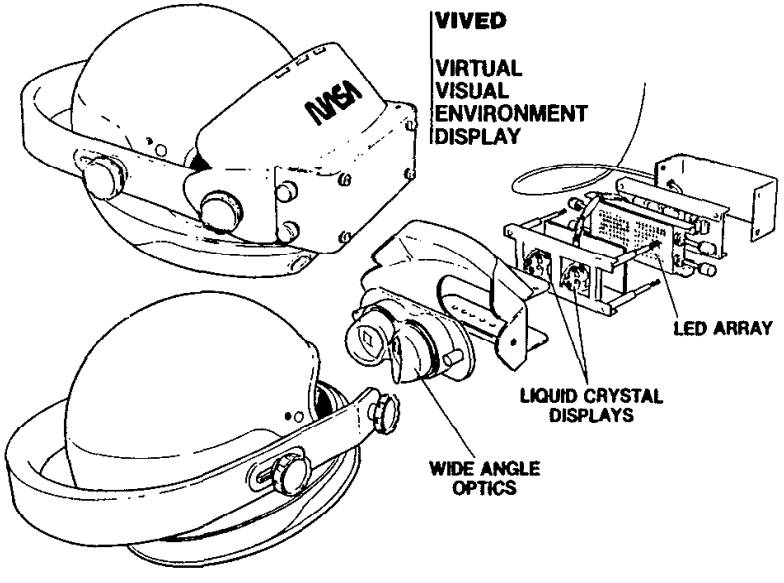
\includegraphics[width=4cm]{FirstVrConcept}\label{fig:FirstVrConcept}}}%
    \qquad
    \subfloat[Sicht auf einen VIVED Benutzer]{{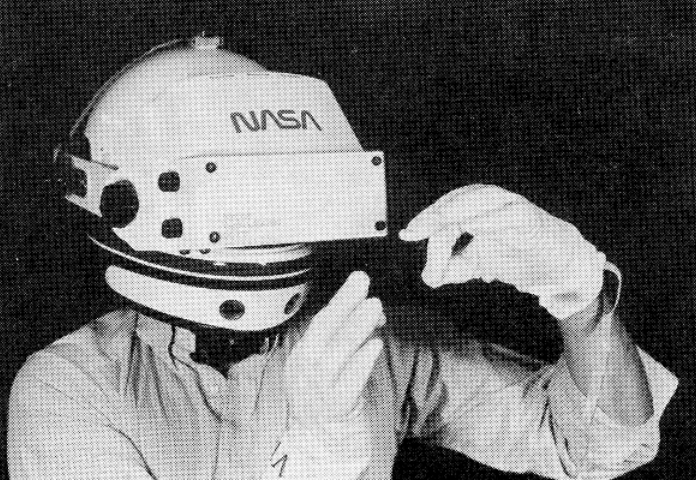
\includegraphics[width=4cm]{FirstVrOutsideView}\label{fig:FirstVrOutsideView}}}%
    \qquad
    \subfloat[Sicht eines VIVED Benutzers]{{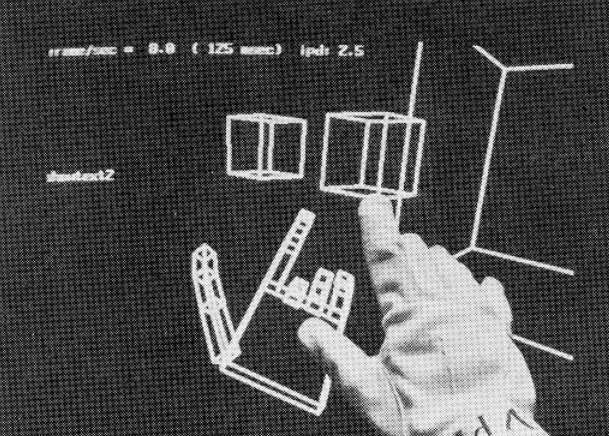
\includegraphics[width=4cm]{FirstVrUserView}\label{fig:FirstVrUserView}}}%
    \qquad
    \subfloat[Rift Displayaufbau \cite{bib:RiftReview}]{{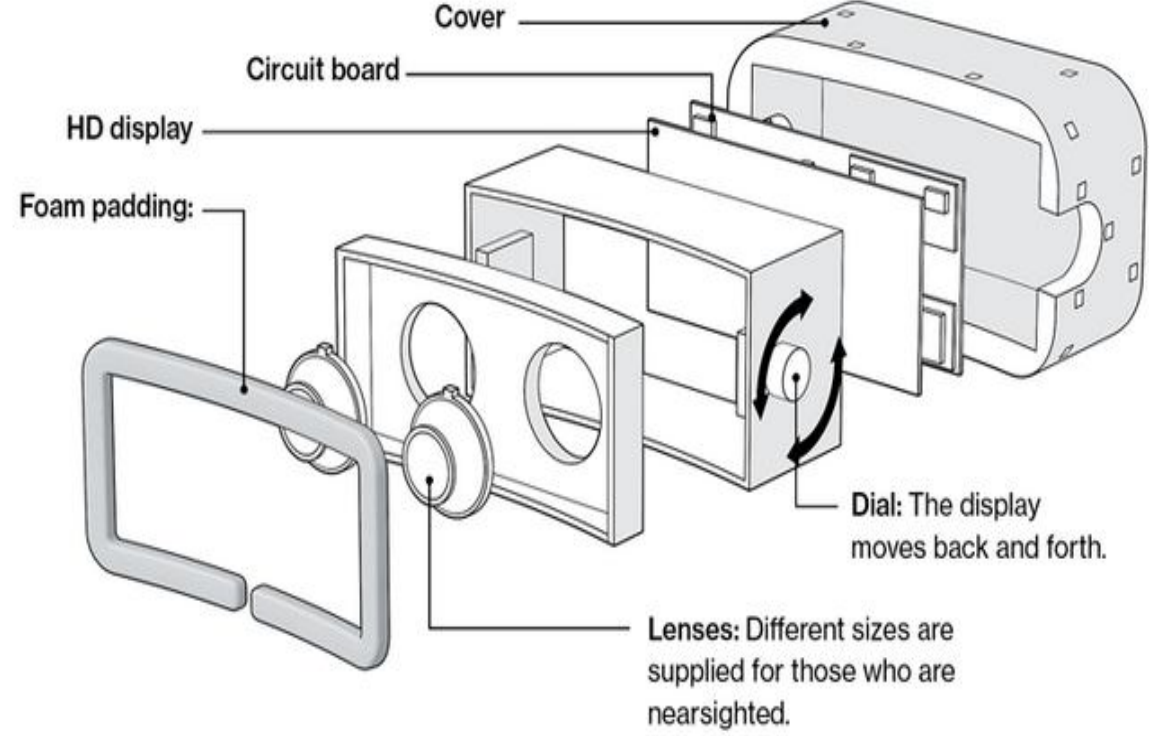
\includegraphics[width=4cm]{RiftConstruction}\label{fig:RiftConstruction}}}%
    \qquad
    \subfloat[Sicht auf einen Rift Benutzer \cite{bib:RiftUser}]{{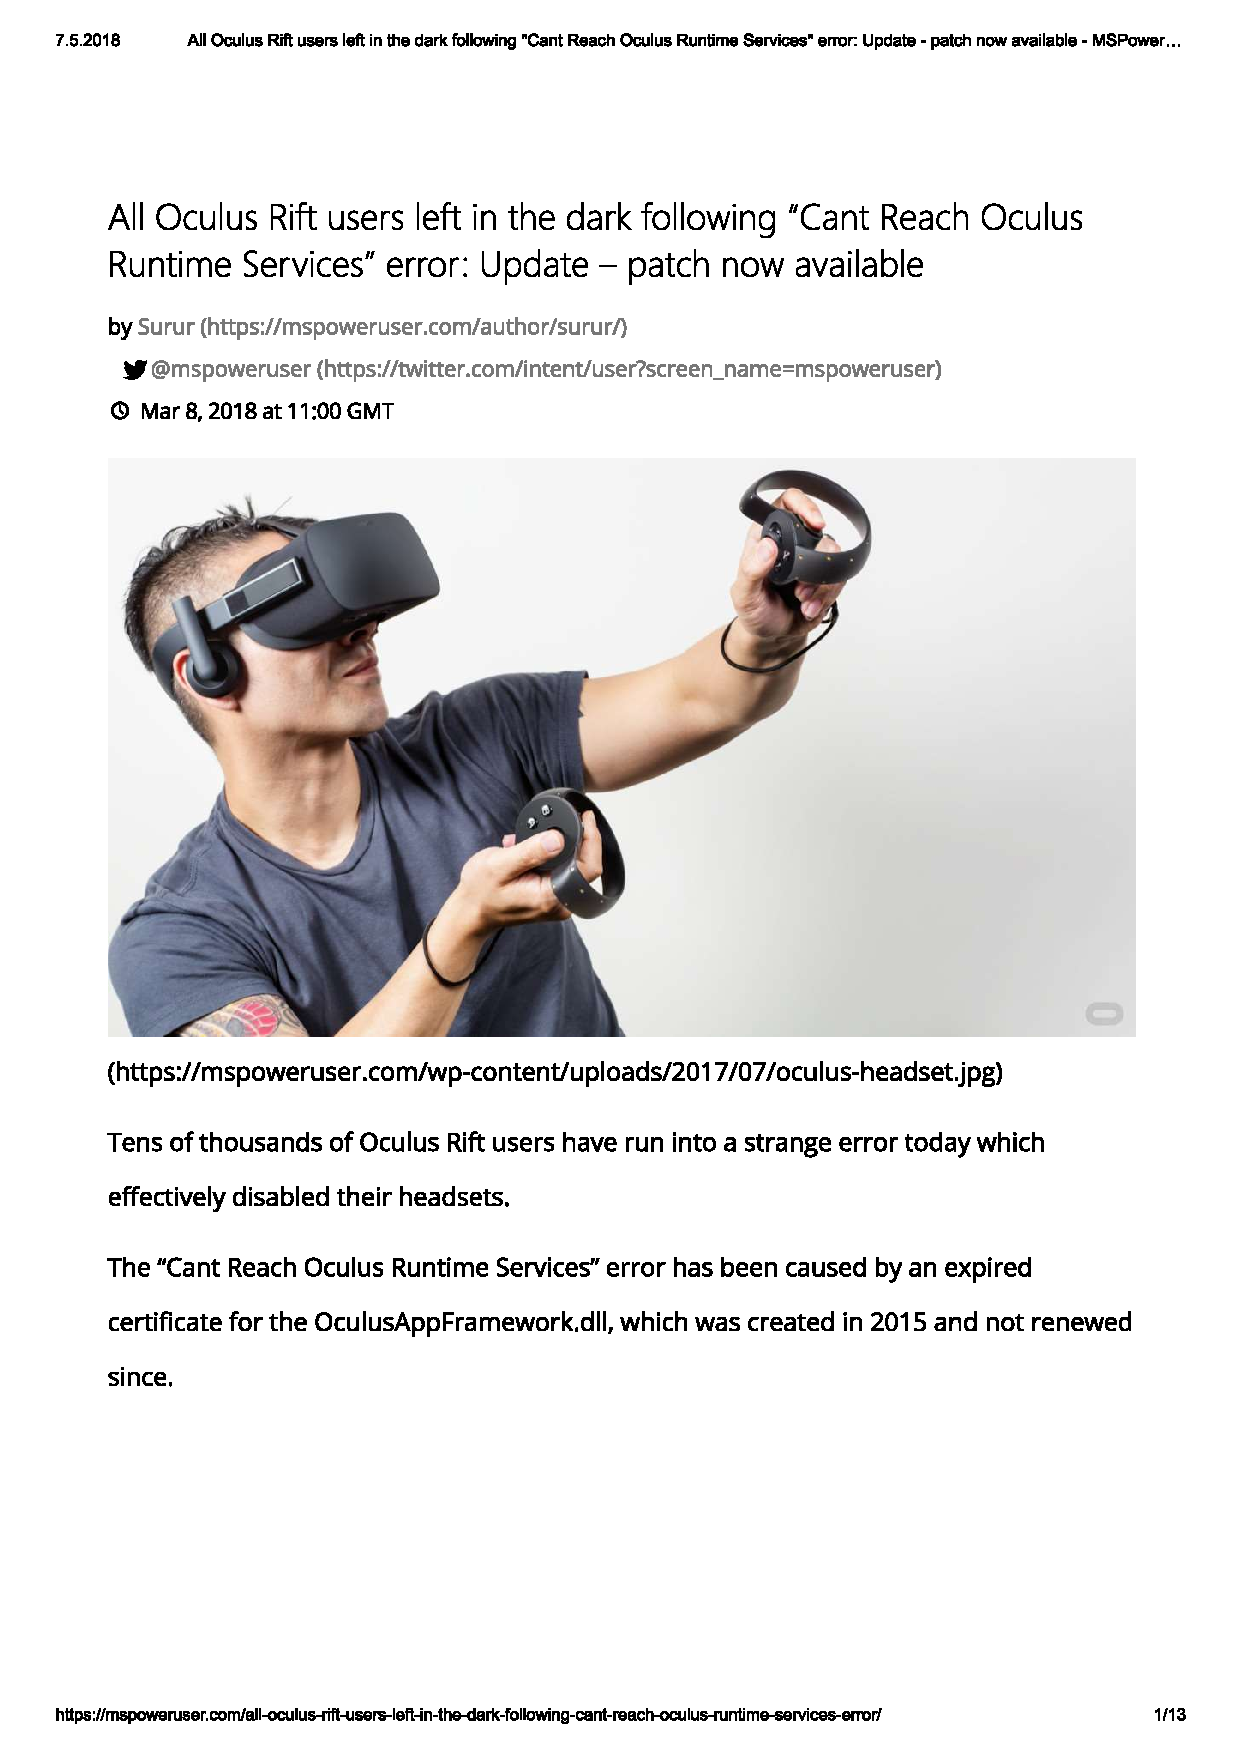
\includegraphics[width=4cm]{RiftUser}\label{fig:RiftUser}}}%
    \qquad
    \subfloat[Sicht eines Rift Benutzers \cite{bib:AvatarHands}]{{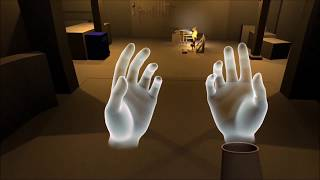
\includegraphics[width=4cm]{RiftAvatar}\label{fig:RiftAvatar}}}%
    \caption{Vergleich zwischen den Anfängen der VR-Technologie und dem heutigen Stand. Die oberen drei Bilder zeigen das VIVED-System, das von S.S. Fisher vorgestellt wurde \cite{bib:NasaVr}. Die Unteren zeigen Bilder der Oculus Rift.}\label{fig:VIVED}%
\end{figure}

Die funktionelle Leistung der Komponenten ist im Laufe der Zeit jedoch deutlich besser geworden. Statt eckigen Polygonen können nun hochauflösende 3D-Modelle durch ein Display mit 2160 x 1200 Pixeln dargestellt werden (Abbildung \ref{fig:RiftAvatar}). Die Brille und die Eingabegeräte werden nun auch, zusätzlich zu den internen Bewegungssensoren, von externen Infrarot-Sensoren erfasst, um eine präzise Portierung der physischen Bewegungen in virtuelle zu übersetzen. Der größte Unterschied ist wohl, dass die VR-Technologie heutzutage hauptsächlich für Unterhaltungszwecke genutzt wird. Was früher ein Forschungsprojekt einer Raumfahrtorganisation war, ist heute ein Entertainment-System, das in vielen Privathaushalten zu finden ist.\\

Ein Grund dafür war die Entwicklung der zwei, derzeit geläufigsten VR-Brillen \textit{Oculus Rift} und \textit{HTC Vive}. Ein paar geschichtliche Eckdaten davon wurden in \cite{bib:RiftHistorical} gesammelt. 2010 wurde der erste Prototyp der Oculus Rift von Palmer Luckily entworfen. Dieser hatte eine horizontale Sichtweite von 90°, was zur damaligen Zeit im Verbrauchermarkt einzigartig war. 2013 hatte Valve einen Durchbruch bei der Entwicklung von \textit{Low-Persistence}-Displays, den sie öffentlich geteilt haben. Dies war sehr hilfreich für alle Entwickler von VR-Brillen. Oculus beispielsweise benutzte diese Art Display bei all ihren nachfolgenden Geräten. Low-Persistence (zu deutsch: \textit{geringe Ausdauer}) bedeutet in dem Falle die angezeigten Bilder nur wenige Millisekunden anzuzeigen, um somit Objekte, die sich Bewegen schärfer darstellen zu können. 2014 wurde Oculus Rift für zwei Milliarden Dollar von Facebook gekauft und beschäftigen mittlerweile circa 400 Mitarbeiter allein für die Virtual Reality Entwicklung. Daran kann man das Potential sehen, das große Konzerne in der VR-Technologie sehen, denn kurz danach kündigte nämlich auch Sony eine VR-Brille für die Playstation 4 an.\\

Die, aus der Großproduktion der führenden VR-Konzerne resultierende, Massentauglichkeit und die Erschwinglichkeit der Technologie machen diese aber auch für die Industrie interessant. Vor allem Im Zuge der \textit{Industrie 4.0} ist VR für Digitalisierung des industriellen Umfelds von Nutzen. Es werden Leistungsfähige und qualitativ immer bessere Lösungen zur virtuellen Datenerfassung und -visualisierung entwickelt. Mittels VR lassen sich Arbeitssituationen simulieren und gefahrlos testen. Industriearbeiter können in Umgebungen agieren, die in der Form noch gar nicht existieren. So können zum Beispiel Arbeitsumfelder und -prozesse effizient geplant werden. Schadens- und Störfälle lassen sich dank VR schnell und in Gänze erfassen und aus der Ferne warten. Es können auch Dinge räumlich begehbar gemacht werden, die es in der physischen Welt nicht gibt, wie beispielsweise Sensordaten. Im Rahmen dieser Arbeit werden Daten eines Lidarsensors als Punktwolke dargestellt, durch die man sich dann Bewegen kann.  




